%%%%%%%%%%%%%%%% Amandine
\section{Dataset}
\begin{frame}[c]
    \begin{figure}
        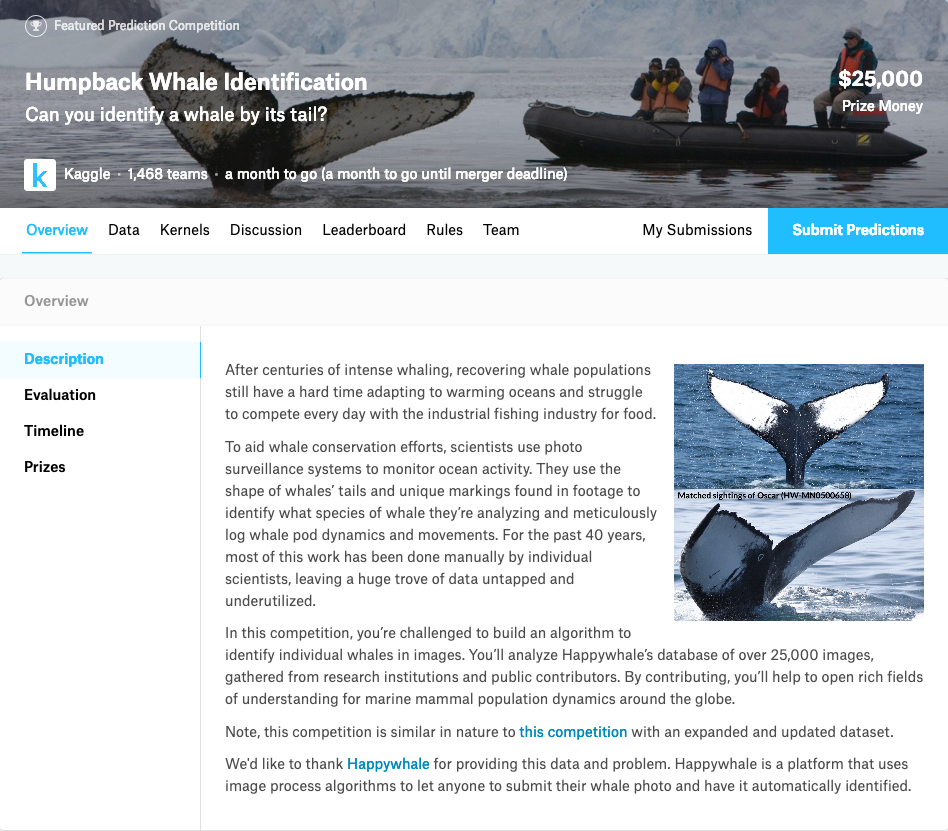
\includegraphics[width=\linewidth]{Kaggle.png}
        \captionsetup{labelformat=empty}
        \caption{}
    \end{figure}
\end{frame}

%%%%%%%%%%%%%%%% Amandine
\begin{frame}[c]
    \begin{figure}
        \centering
        \begin{subfigure}[b]{0.24\linewidth}
            \centering
            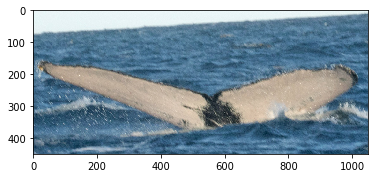
\includegraphics[width=\linewidth]{Whales/new_whale0.png}
            \caption{Ophélie}
        \end{subfigure}
        \begin{subfigure}[b]{0.24\linewidth}
            \centering
            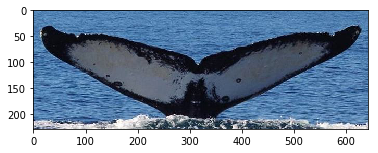
\includegraphics[width=\linewidth]{Whales/new_whale4.png}
            \caption{Alexis}
        \end{subfigure}
        \begin{subfigure}[b]{0.24\linewidth}
            \centering
            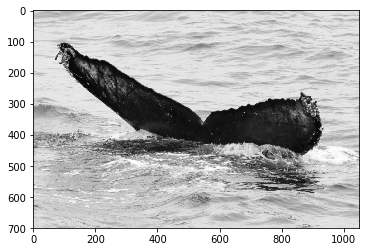
\includegraphics[width=\linewidth]{Whales/w_6310ac7.png}
            \caption{Antoine}
        \end{subfigure}
        \begin{subfigure}[b]{0.24\linewidth}
            \centering
            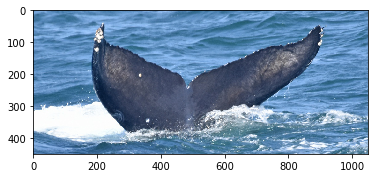
\includegraphics[width=\linewidth]{Whales/w_9a5bb2d.png}
            \caption{Florian}
        \end{subfigure}
        \begin{subfigure}[b]{0.24\linewidth}
            \centering
            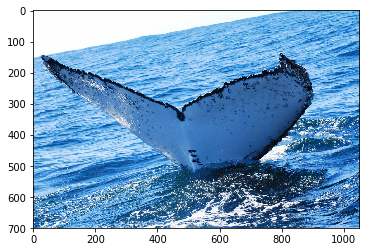
\includegraphics[width=\linewidth]{Whales/new_whale1.png}
            \caption{Jules}
        \end{subfigure}
        \begin{subfigure}[b]{0.24\linewidth}
            \centering
            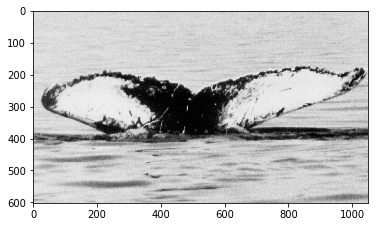
\includegraphics[width=\linewidth]{Whales/new_whale5.png}
            \caption{Benedicte}
        \end{subfigure}
        \begin{subfigure}[b]{0.24\linewidth}
            \centering
            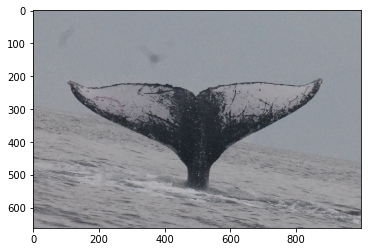
\includegraphics[width=\linewidth]{Whales/w_73e5b74.png}
            \caption{Apolline}
        \end{subfigure}
        \begin{subfigure}[b]{0.24\linewidth}
            \centering
            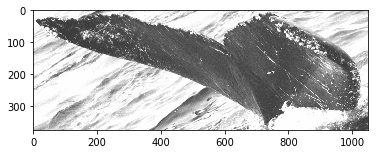
\includegraphics[width=\linewidth]{Whales/w_b9e5911.png}
            \caption{Julie}
        \end{subfigure}
        \begin{subfigure}[b]{0.24\linewidth}
            \centering
            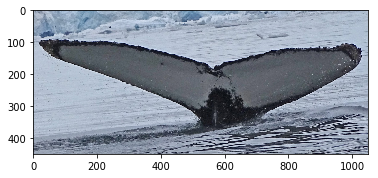
\includegraphics[width=\linewidth]{Whales/new_whale2.png}
            \caption{Ibrahima}
        \end{subfigure}
        \begin{subfigure}[b]{0.24\linewidth}
            \centering
            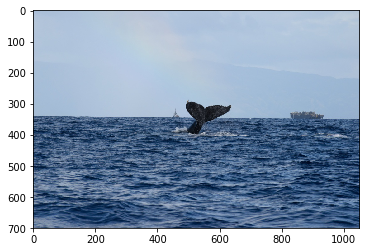
\includegraphics[width=\linewidth]{Whales/new_whale6.png}
            \caption{Grégoire}
        \end{subfigure}
        \begin{subfigure}[b]{0.24\linewidth}
            \centering
            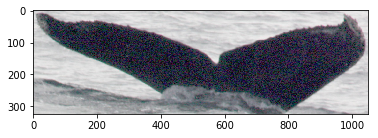
\includegraphics[width=\linewidth]{Whales/w_84308d6.png}
            \caption{Yasser}
        \end{subfigure}
        \begin{subfigure}[b]{0.24\linewidth}
            \centering
            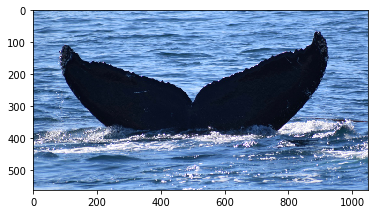
\includegraphics[width=\linewidth]{Whales/w_e1ffbe2.png}
            \caption{Aurelien}
        \end{subfigure}
        \begin{subfigure}[b]{0.24\linewidth}
            \centering
            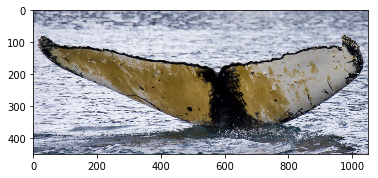
\includegraphics[width=\linewidth]{Whales/new_whale3.png}
            \caption{Clara}
        \end{subfigure}
        \begin{subfigure}[b]{0.24\linewidth}
            \centering
            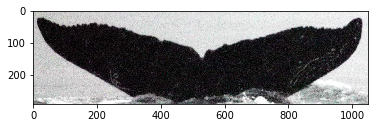
\includegraphics[width=\linewidth]{Whales/w_5101888.png}
            \caption{Dimitri}
        \end{subfigure}
        \begin{subfigure}[b]{0.24\linewidth}
            \centering
            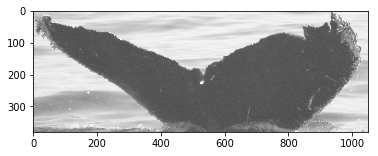
\includegraphics[width=\linewidth]{Whales/w_865cf80.png}
            \caption{Fahmi}
        \end{subfigure}
        \begin{subfigure}[b]{0.24\linewidth}
            \centering
            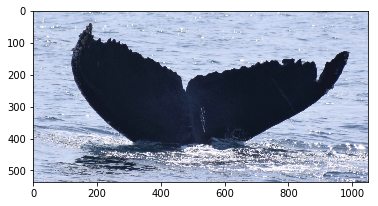
\includegraphics[width=\linewidth]{Whales/w_f6c5343.png}
            \caption{Nataliya}
        \end{subfigure}
    \end{figure}
\end{frame}

%%%%%%%%%%%%%%%% Amandine
\begin{frame}[c]
    \begin{figure}
        \centering
        \begin{subfigure}[b]{0.24\linewidth}
            \centering
            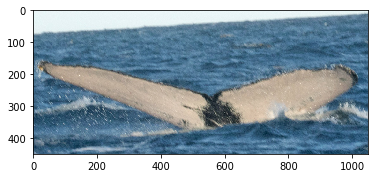
\includegraphics[width=\linewidth]{Whales/new_whale0.png}
            \caption{new\_whale}
        \end{subfigure}
        \begin{subfigure}[b]{0.24\linewidth}
            \centering
            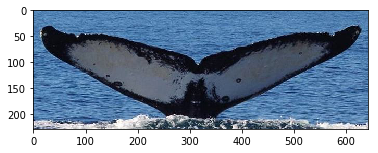
\includegraphics[width=\linewidth]{Whales/new_whale4.png}
            \caption{new\_whale}
        \end{subfigure}
        \begin{subfigure}[b]{0.24\linewidth}
            \centering
            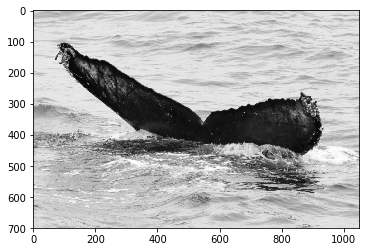
\includegraphics[width=\linewidth]{Whales/w_6310ac7.png}
            \caption{w\_6310ac7}
        \end{subfigure}
        \begin{subfigure}[b]{0.24\linewidth}
            \centering
            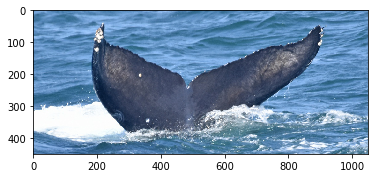
\includegraphics[width=\linewidth]{Whales/w_9a5bb2d.png}
            \caption{w\_9a5bb2d}
        \end{subfigure}
        \begin{subfigure}[b]{0.24\linewidth}
            \centering
            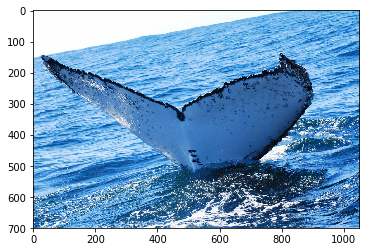
\includegraphics[width=\linewidth]{Whales/new_whale1.png}
            \caption{new\_whale}
        \end{subfigure}
        \begin{subfigure}[b]{0.24\linewidth}
            \centering
            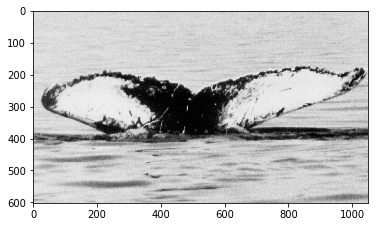
\includegraphics[width=\linewidth]{Whales/new_whale5.png}
            \caption{new\_whale}
        \end{subfigure}
        \begin{subfigure}[b]{0.24\linewidth}
            \centering
            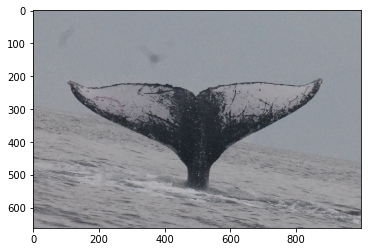
\includegraphics[width=\linewidth]{Whales/w_73e5b74.png}
            \caption{w\_73e5b74}
        \end{subfigure}
        \begin{subfigure}[b]{0.24\linewidth}
            \centering
            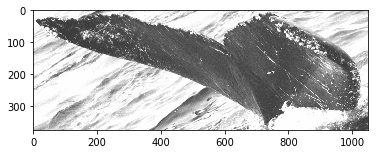
\includegraphics[width=\linewidth]{Whales/w_b9e5911.png}
            \caption{w\_b9e5911}
        \end{subfigure}
        \begin{subfigure}[b]{0.24\linewidth}
            \centering
            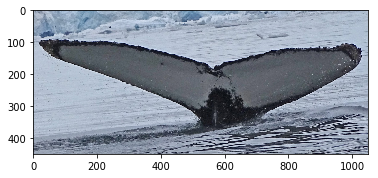
\includegraphics[width=\linewidth]{Whales/new_whale2.png}
            \caption{new\_whale}
        \end{subfigure}
        \begin{subfigure}[b]{0.24\linewidth}
            \centering
            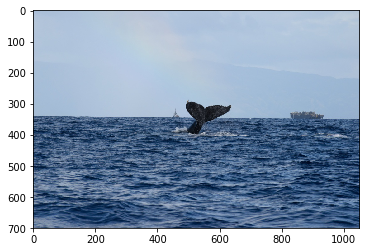
\includegraphics[width=\linewidth]{Whales/new_whale6.png}
            \caption{new\_whale}
        \end{subfigure}
        \begin{subfigure}[b]{0.24\linewidth}
            \centering
            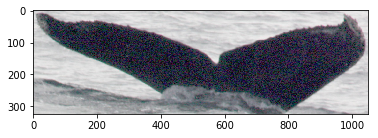
\includegraphics[width=\linewidth]{Whales/w_84308d6.png}
            \caption{w\_84308d6}
        \end{subfigure}
        \begin{subfigure}[b]{0.24\linewidth}
            \centering
            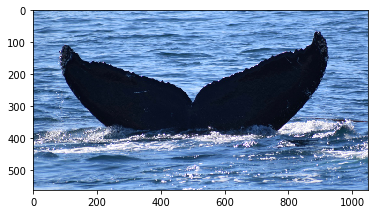
\includegraphics[width=\linewidth]{Whales/w_e1ffbe2.png}
            \caption{w\_e1ffbe2}
        \end{subfigure}
        \begin{subfigure}[b]{0.24\linewidth}
            \centering
            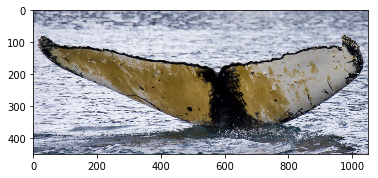
\includegraphics[width=\linewidth]{Whales/new_whale3.png}
            \caption{new\_whale}
        \end{subfigure}
        \begin{subfigure}[b]{0.24\linewidth}
            \centering
            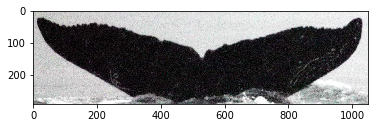
\includegraphics[width=\linewidth]{Whales/w_5101888.png}
            \caption{w\_5101888}
        \end{subfigure}
        \begin{subfigure}[b]{0.24\linewidth}
            \centering
            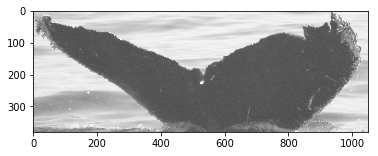
\includegraphics[width=\linewidth]{Whales/w_865cf80.png}
            \caption{w\_865cf80}
        \end{subfigure}
        \begin{subfigure}[b]{0.24\linewidth}
            \centering
            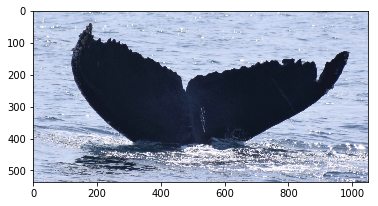
\includegraphics[width=\linewidth]{Whales/w_f6c5343.png}
            \caption{w\_f6c5343}
        \end{subfigure}
    \end{figure}
\end{frame}

%%%%%%%%%%%%%%%% Amandine
\begin{frame}[c]{Dataset}
    The \url{happywhale.com} dataset in numbers:
    \begin{center}
    \begin{itemize}
        \item \texttt{input/train/} (\Large{\textbf{4,55 GB}} on disk) for \textbf{25 362} items
        \large \item \texttt{input/test/} (\large{\textbf{1,47 GB}} on disk) for \textbf{7 961} items
    \end{itemize}
    \end{center}
\end{frame}

%%%%%%%%%%%%%%%% Yvan
\begin{frame}
% Pour créer le suspens ...
\end{frame}

\section{Score}
\begin{frame}[c]
    \Huge \texttt{SCORE = 0.314}
    \newline\newline
    \tiny \emph{Is it a good score?} % TODO
\end{frame}

%%%%%%%%%%%%%%%% Yvan
\begin{frame}[c]{Mean Average Precision (MAP)}
    Submissions are evaluated according to the \emph{Mean Average Precision
    \texttt{@5}} (\texttt{MAP@5}):
    $$MAP@5 = \frac{1}{U} \sum_{u=1}^{U}  \sum_{k=1}^{min(n,5)} P(k)$$
    where $U$ is the number of images, $P(k)$ is the precision at cutoff $k$, and
    $n$ is the number predictions per image.
\end{frame}

\begin{frame}[c]{Precision}
    Precision (also called positive predictive value) is the fraction of
    relevant instances among the retrieved instances.
    
    In a classification task, the precision for a class is the number of
    true positives (\emph{i.e.} the number of items correctly labeled as belonging
    to the positive class) divided by the total number of elements labeled
    as belonging to the positive class (\emph{i.e.} the sum of true positives and
    false positives, which are items incorrectly labeled as belonging to the
    class).
    
    $$P = { \#\ of\ correct\ predictions\over \#\ of\ all\ predictions  } = {TP \over (TP + FP)}$$
\end{frame}

%%%%%%%%%%%%%%%% Yvan
\begin{frame}[c]{Precision \texttt{@k}}
    Precision at cutoff $k$, $P(k)$, is simply the precision
    calculated by considering only the subset of your predictions from rank
    1 through $k$. For example:
    
    \begin{longtable}[]{@{}cccc@{}}
    \toprule
    true & predicted & k & P(k)\tabularnewline
    \midrule
    \endhead
    {[}x{]} & {[}0, ?, ?, ?, ?{]} & 1 & 0/1 = \textbf{0}\tabularnewline
    {[}x{]} & {[}\textbf{1}, ?, ?, ?, ?{]} & 1 & 1/1 = \textbf{1}\tabularnewline
    {[}x{]} & {[}\textbf{1}, 0, ?, ?, ?{]} & 2 & 1/1 + 0/2 = \textbf{1}\tabularnewline
    {[}x{]} & {[}0, \textbf{1}, ?, ?, ?{]} & 2 & 0/1 + 1/2 = \textbf{1/2}\tabularnewline
    {[}x{]} & {[}\textbf{1}, \textbf{1}, ?, ?, ?{]} & 2 & 1/1 + 1/2 = \textbf{3/2}\tabularnewline
    \bottomrule
    \end{longtable}
    
    where \texttt{1} is a correct prediction, \texttt{1} an incorrect prediction and \texttt{?} is either a correct or an incorrect prediction.
\end{frame}

%%%%%%%%%%%%%%%% Yvan
\begin{frame}[c]{Precision \texttt{@5} per image}
    The calculation would stop after the first
    occurrence of the correct whale,
    we don't have to sum up to 5, only up to the first correct answer. In
    this competition there is only one correct answer per
    image, so the possible precision scores per image are $1/k$ for $k \in \{1, 2, 3, 4, 5\}$:
    
    \begin{longtable}[]{@{}ccccc@{}}
    \toprule
    true & predicted & k & Image score &\tabularnewline
    \midrule
    \endhead
    {[}x{]} & {[}\textbf{1}, ?, ?, ?, ?{]} & 5 & \textbf{1} &\tabularnewline
    {[}x{]} & {[}0, \textbf{1}, ?, ?, ?{]} & 5 & \textbf{1/2} &\tabularnewline
    {[}x{]} & {[}0, 0, \textbf{1}, ?, ?{]} & 5 & \textbf{1/3} &\tabularnewline
    {[}x{]} & {[}0, 0, 0, \textbf{1}, ?{]} & 5 & \textbf{1/4} &\tabularnewline
    {[}x{]} & {[}0, 0, 0, 0, \textbf{1}{]} & 5 & \textbf{1/5} &\tabularnewline
    {[}x{]} & {[}0, 0, 0, 0, 0{]} & 5 & \textbf{0} &\tabularnewline
    \bottomrule
    \end{longtable}
    
    \textbf{Leaderboard score}: The final score is simply the average over the scores of all the images.
\end{frame}

%%%%%%%%%%%%%%%% Yvan
\begin{frame}[c]{What's \texttt{MAP@5} score of a \textbf{random} prediction ?!}
    \begin{center}
    With $P(k) = \frac{1}{C} \times \frac{1}{k}$ \emph{(random)}:
    $$MAP@5(U) = \textcolor{red}{\frac{1}{U} \sum_{u=1}^{U}} \Big( \sum_{k=1}^{min(n,5)} P(k) \Big) \leqslant \frac{1}{C} \textcolor{blue}{\sum_{k=1}^5 \frac{1}{k}} = \frac{1}{C} \textcolor{blue}{\frac{137}{60}}$$
    \newline\newline
    For $C = 5005$ (\# of classes in our test dataset)
    \newline\newline
    $MAP@5(U) \leqslant$ \textbf{0.000456}
    \newline\newline
    \tiny \emph{Okay, 0.314 does not seem too bad!}
    \end{center}
\end{frame}

\section{Pipeline overview}
%%%%%%%%%%%%%%%% Amandine
\begin{frame}[c]
    \begin{figure}
        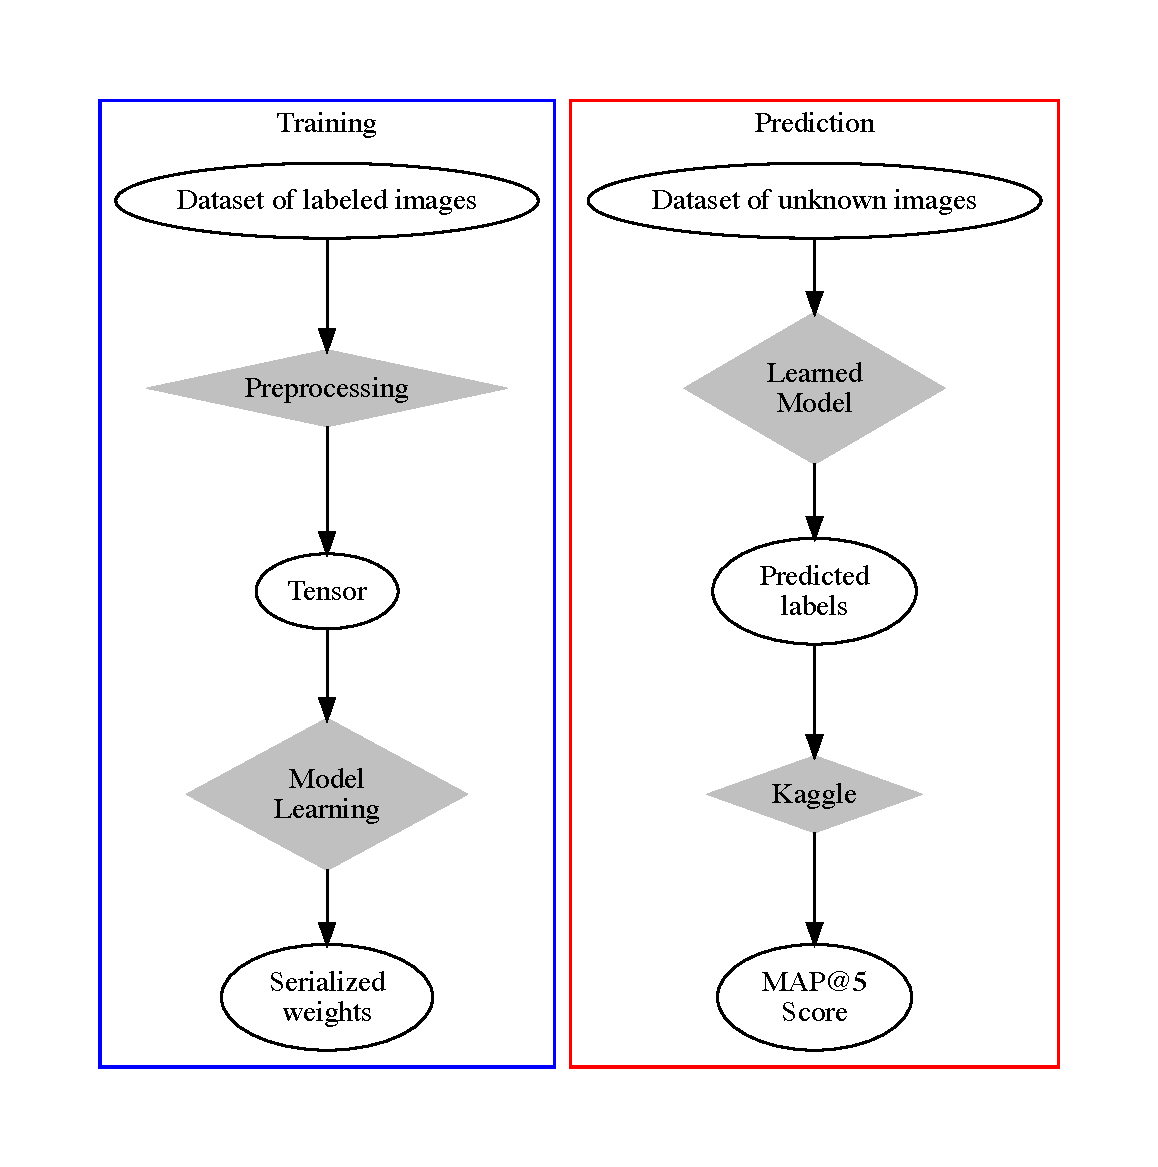
\includegraphics[width=0.75\linewidth]{flowchart.pdf}
        \caption{Flowchart of our pipeline}
    \end{figure}
\end{frame}

%%%%%%%%%%%%%%%% Amandine
\begin{frame}[c]{Benchmark of preprocessing methods}
    \begin{table}[]
    \begin{tabular}{ll}
                                                 & \textbf{Score}\\
    \texttt{128x128} unaltered images            & 0,290 \\
    \textbf{Experience 1}                        &       \\
    \texttt{128x128} black and white             & 0,289 \\
    \texttt{128x128} high contrast               & 0,288 \\
    \textbf{Experience 2}                        &       \\
    \texttt{new\_whale} as a class               & -     \\
    discriminate \texttt{new\_whale} by accuracy & -     \\
    \textbf{Experience 3}                        &       \\
    bounding box                                 & -
    \end{tabular}
    \end{table}
\end{frame}

%%%%%%%%%%%%%%%% Yvan
\subsection{A priori}
\begin{frame}[c]{\emph{A priori}: ``A whale is not a fire truck?''}
    \begin{figure}
        \centering
        \begin{subfigure}[b]{0.4\linewidth}
            \centering
            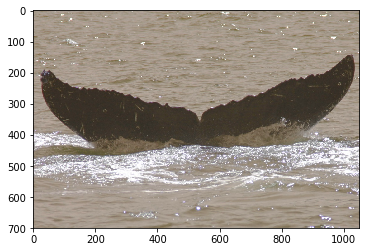
\includegraphics[width=\linewidth]{normal.png}
            \caption{Whale}
        \end{subfigure}
        \begin{subfigure}[b]{0.4\linewidth}
            \centering
            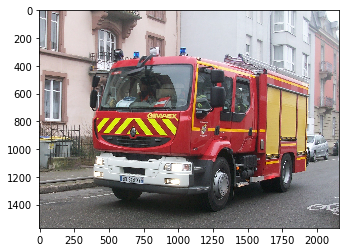
\includegraphics[width=\linewidth]{firetruck.png}
            \caption{Fire truck}
        \end{subfigure}
        \caption{Colors could help identify fire trucks in a dataset of vehicules!}
    \end{figure}
\end{frame}

%%%%%%%%%%%%%%%% Yvan
\begin{frame}[c]{\emph{A priori}: ``We don't care about colors!''}
    \begin{figure}
        \centering
        \begin{subfigure}[b]{0.4\linewidth}
            \centering
            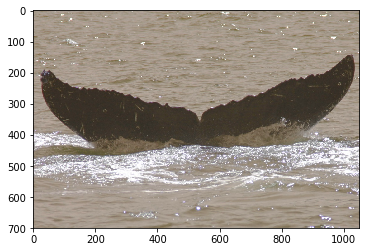
\includegraphics[width=\linewidth]{normal.png}
            \caption{Whale}
        \end{subfigure}
        \begin{subfigure}[b]{0.4\linewidth}
            \centering
            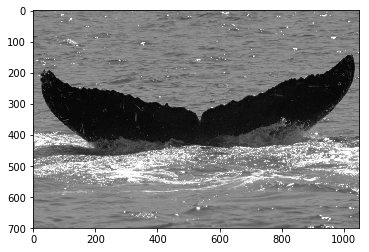
\includegraphics[width=\linewidth]{black_and_white.png}
            \caption{Whale (black and white)}
        \end{subfigure}
        \caption{Learn colors in whale identification would be \textbf{overfitting}!}
        We check that our model do not loose accuracy by this transformation. As a bonus, we reduce by 3 the size of our tensor.
    \end{figure}
\end{frame}

%%%%%%%%%%%%%%%% Yvan
\subsection{Image pre-processing}
\begin{frame}[c]{Image and label preprocessing}
    \Large
    %Pre-processing : change the shape of the image and convert them
    %to an array (tensor)
    \begin{itemize}
    \tightlist
    \item \textbf{Tensor}: resized image encoded in vector of \texttt{128x128} weights $w_i$, with $w_i \in [0, 1]$, $\forall i \in [0..128\times128]$
    \item \textbf{Encoding}: $f: c \to i$ with $c \in Classes$ and $i \in \mathbb{N}$ ($f$ \emph{bijective})
    \end{itemize}
\end{frame}

%%%%%%%%%%%%%%%% Yvan
\subsection{A priori}
\begin{frame}[c]{\emph{A priori}: ``Bigger images is better''}
    \begin{figure}
        \centering
        \begin{subfigure}[b]{0.4\linewidth}
            \centering
            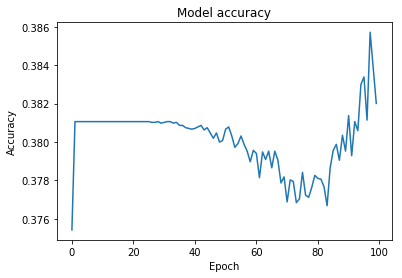
\includegraphics[width=\linewidth]{16x16.png}
            \caption{16x16}
        \end{subfigure}
        \begin{subfigure}[b]{0.4\linewidth}
            \centering
            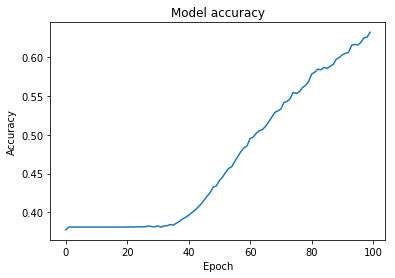
\includegraphics[width=\linewidth]{32x32.png}
            \caption{32x32}
        \end{subfigure}
        \begin{subfigure}[b]{0.4\linewidth}
            \centering
            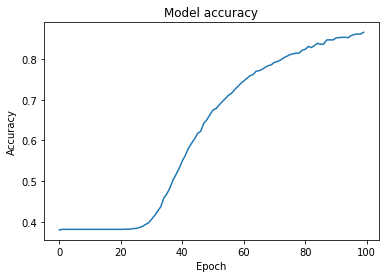
\includegraphics[width=\linewidth]{64x64.png}
            \caption{64x64}
        \end{subfigure}
        \begin{subfigure}[b]{0.4\linewidth}
            \centering
            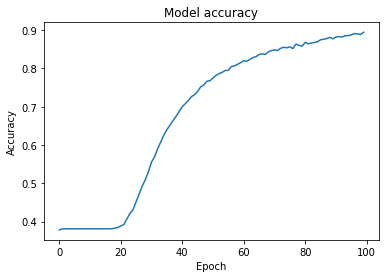
\includegraphics[width=\linewidth]{128x128.png}
            \caption{128x128}
        \end{subfigure}
        \caption{The learned model accuracy seems to increase with image size!}
    \end{figure}
\end{frame}

%%%%%%%%%%%%%%%% Yvan
\begin{frame}[c]{\texttt{"new\_whale"} class bias}
    \Large
    \begin{table}[]
    \begin{tabular}{ll}
    \textbf{class} & \textbf{\#}\\
    \textcolor{red}{new\_whale} &   \textcolor{red}{9664} \\
    w\_23a388d &     73 \\
    w\_9b5109b &     65 \\
    w\_9c506f6 &     62 \\
    w\_0369a5c &     61
    \end{tabular}
    \end{table}
    \normalsize Score obtained with \texttt{["new\_whale", "new\_whale", "new\_whale", "new\_whale", "new\_whale"]} for all predictions on test dateset is \textbf{0.276}!
\end{frame}

%%%%%%%%%%%%%%%% Yvan
\begin{frame}[c]{Bounding box}
    \begin{figure}
        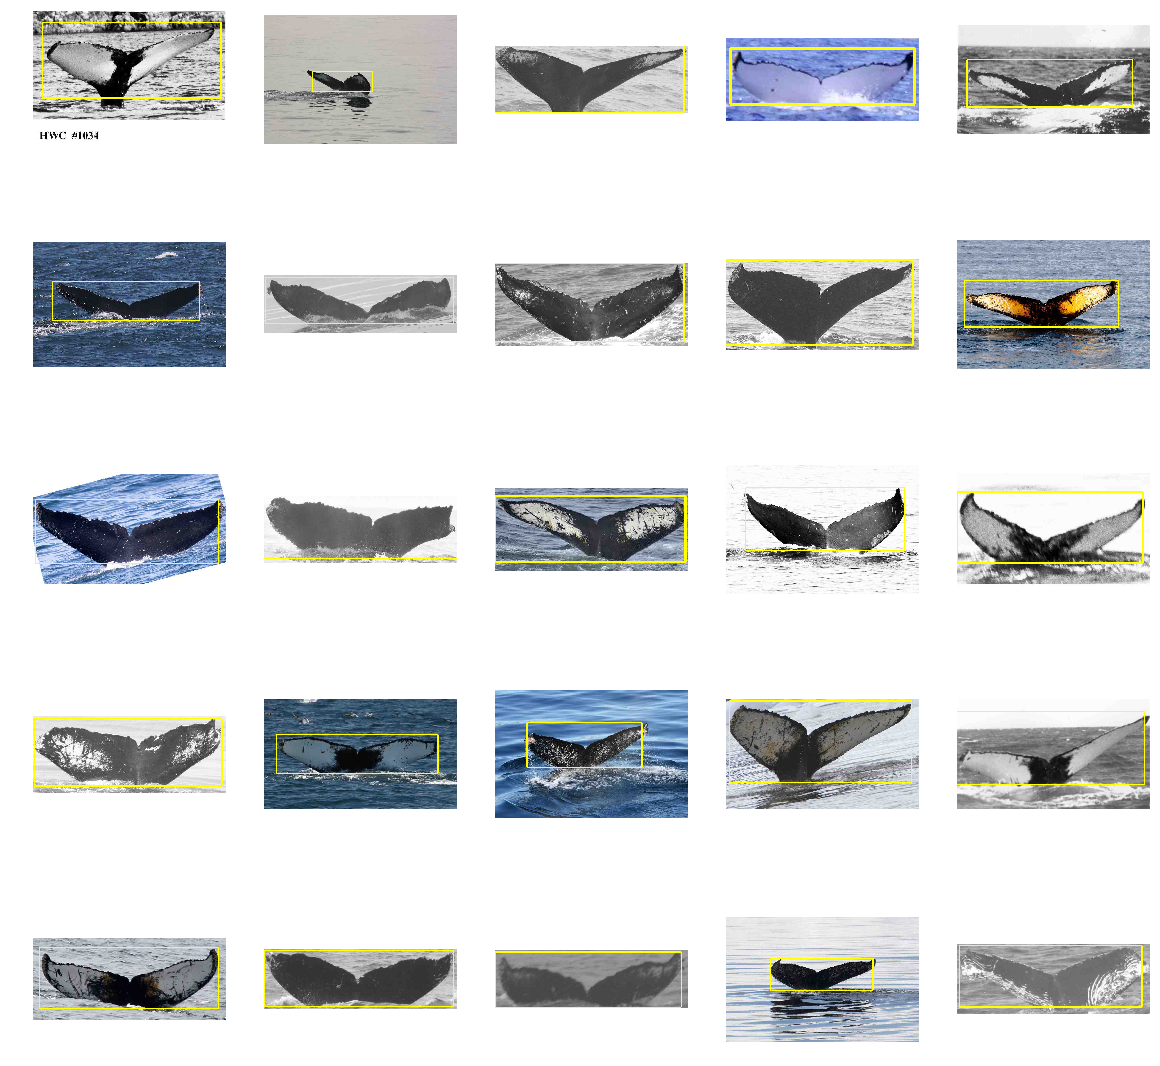
\includegraphics[width=\linewidth]{bounding-box.png}
        \captionsetup{labelformat=empty}
        \caption{}
    \end{figure}
\end{frame}

%%%%%%%%%%%%%%%% Amandine
\subsection{Learning method} 
\begin{frame}[c]{Learning method}
    We choose to use \textbf{Convolutional Neural Networks} (CNN) which is well known\cite{NIPS2012_4824} to be one of the first class machine learning algorithm for general purpose image classification.
    \newline\newline
    \textbf{Why we do not try something like:}
    \begin{itemize}
        \item Boosting?
        \item Random Forests?
        \item SVM?
        \item ...
    \end{itemize}
\end{frame}

%%%%%%%%%%%%%%%% Amandine
\begin{frame}[c]
    \textbf{What is the issue with classical machine learning methods on images?} \emph{e.g.:}
    \begin{figure}
        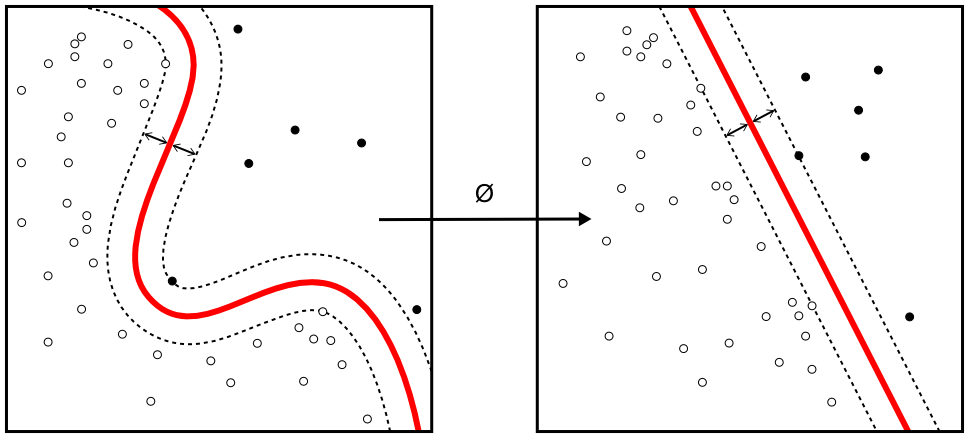
\includegraphics[width=\linewidth]{Kernel_Machine.png}
        \caption{Kernel Machine (SVM)}
   \end{figure}
\end{frame}

%%%%%%%%%%%%%%%% Yvan
\begin{frame}[c]{The curse of high dimensionality}
    \begin{itemize}
        \item \textbf{Space dimension} of images of \texttt{128x128} pixels = \Large 16 384... \normalsize ($256^{16 384}$ black and white images possibles)
        \item ...but only \Large 25 362 \normalsize  images in train dataset (\textbf{points in space})
    \end{itemize}
    \bigskip
    \Large The image space is \emph{really really really} sparse!
    \newline\newline
    \normalsize We can't assume the hypothesis of the existence of some \textbf{internal structure} in our space and that we can find a \textbf{parsimonious frontier} between our classes.
\end{frame}

%%%%%%%%%%%%%%%% Yvan
\begin{frame}[c]{Invariance by translation}
    \textbf{But images are not just random noise!} They have some internal structure and mathematical properties we can use to reduce (not solve) this issue. \emph{e.g.:}
    \begin{figure}
        \centering
        \begin{subfigure}[b]{0.4\linewidth}
            \centering
            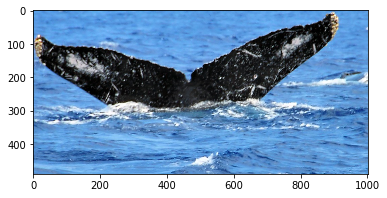
\includegraphics[width=\linewidth]{001.png}
            \captionsetup{labelformat=empty}
            \caption{}
        \end{subfigure}
        \begin{subfigure}[b]{0.4\linewidth}
            \centering
            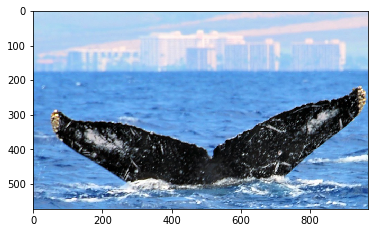
\includegraphics[width=\linewidth]{002.png}
            \captionsetup{labelformat=empty}
            \caption{}
        \end{subfigure}
        \caption{Same image of whale cropped two different ways}
    \end{figure}
    Pixels coordinates are definitely not what we want as dimensions of our images space!
\end{frame}

%%%%%%%%%%%%%%%% Yvan
\begin{frame}[c]{Convolutional Neural Networks}
    A class of \textbf{Deep Neural Network:}
    \begin{itemize}
        \item \textbf{Principle:} list of layers that transform the image volume into an output volume
        \item \textbf{Optimization:} by making incremental adjustments to the biases and weights
    \end{itemize}
    \begin{figure}
        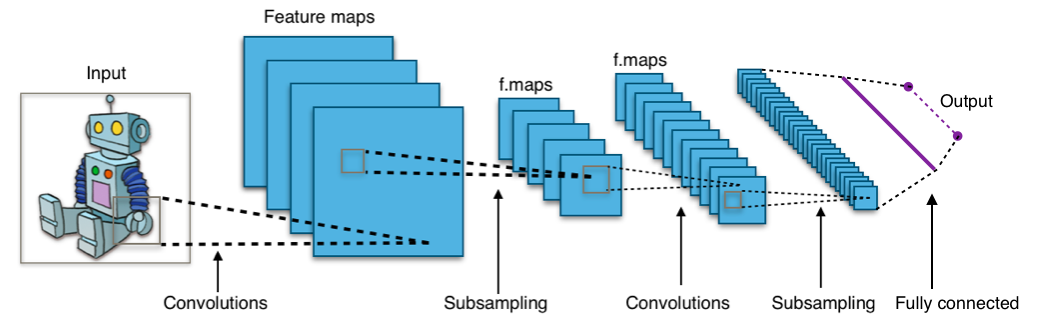
\includegraphics[width=\linewidth]{Typical_cnn.png}
        \caption{a typical CNN}
    \end{figure}
\end{frame}

%%%%%%%%%%%%%%%% Amandine
\begin{frame}[c]{CNN architectures experimentations}
    We try a set of different \textbf{architectures} and \textbf{parameters} for our CNN, here is a small benchmark of tested methods:
    \begin{table}[]
    \begin{tabular}{ll}
    \textbf{Parameters}                 & \textbf{Scores} \\
    Initial parameters & 0.299  \\
    Without dropout & 0,271  \\
    Without batch normalization & 0,303  \\
    With five dense layer & 0,000  \\
    Without activation & 0,257  \\
    With activation layer = \texttt{softmax} & 0,280  \\
    Optimizer = \texttt{SGD} & 0,303  \\
    Optimizer = \texttt{RMSprop} & 0.278  \\
    Optimizer = \texttt{Nadam} & 0.293  \\
    Optimizer = \texttt{Adam} & 0.293  \\
    Optimizer = \texttt{Adadelta} & \textbf{0.314}
    \end{tabular}
    \end{table}
    For performance reasons, we preprocessed images to size \texttt{64x64} in this benchmark.
\end{frame}

%%%%%%%%%%%%%%%% Yvan
\section{Perspectives} 
\begin{frame}[c]{Perspectives}
    \begin{figure}
        \centering
        \begin{subfigure}[b]{0.69\linewidth}
            \centering
            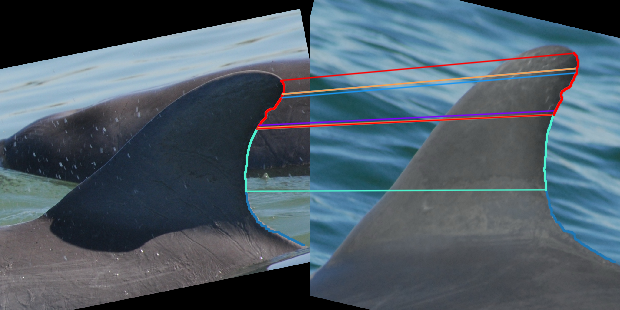
\includegraphics[width=\linewidth]{Weideman2017/014.png}
            \captionsetup{labelformat=empty}
            \caption{}
        \end{subfigure}
        \begin{subfigure}[b]{0.29\linewidth}
            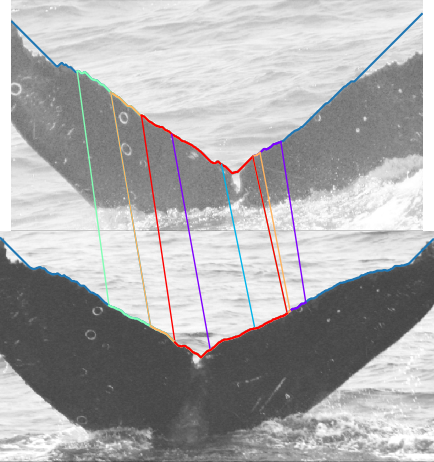
\includegraphics[width=\linewidth]{Weideman2017/026.png}
            \captionsetup{labelformat=empty}
            \caption{}
        \end{subfigure}
        \caption{Integral Curvature Representation and Matching Algorithms \cite{weideman_integral_2017}}
    \end{figure}
\end{frame}

%%%%%%%%%%%%%%%% Yvan
\section{Conclusion} 
    \begin{frame}[c]{Conclusion}
    Literature of \textbf{Convolutional Neural Networks} really show impressive results in various domains of application!
    
    To implement them efficiently still requires a lot of investigations and experimentations, this is not $1^{st}$ grade \emph{``Black Magic''}.

    We lack so much time for experimenting all the methods and parameters we would like.
    \begin{figure}
        \centering
        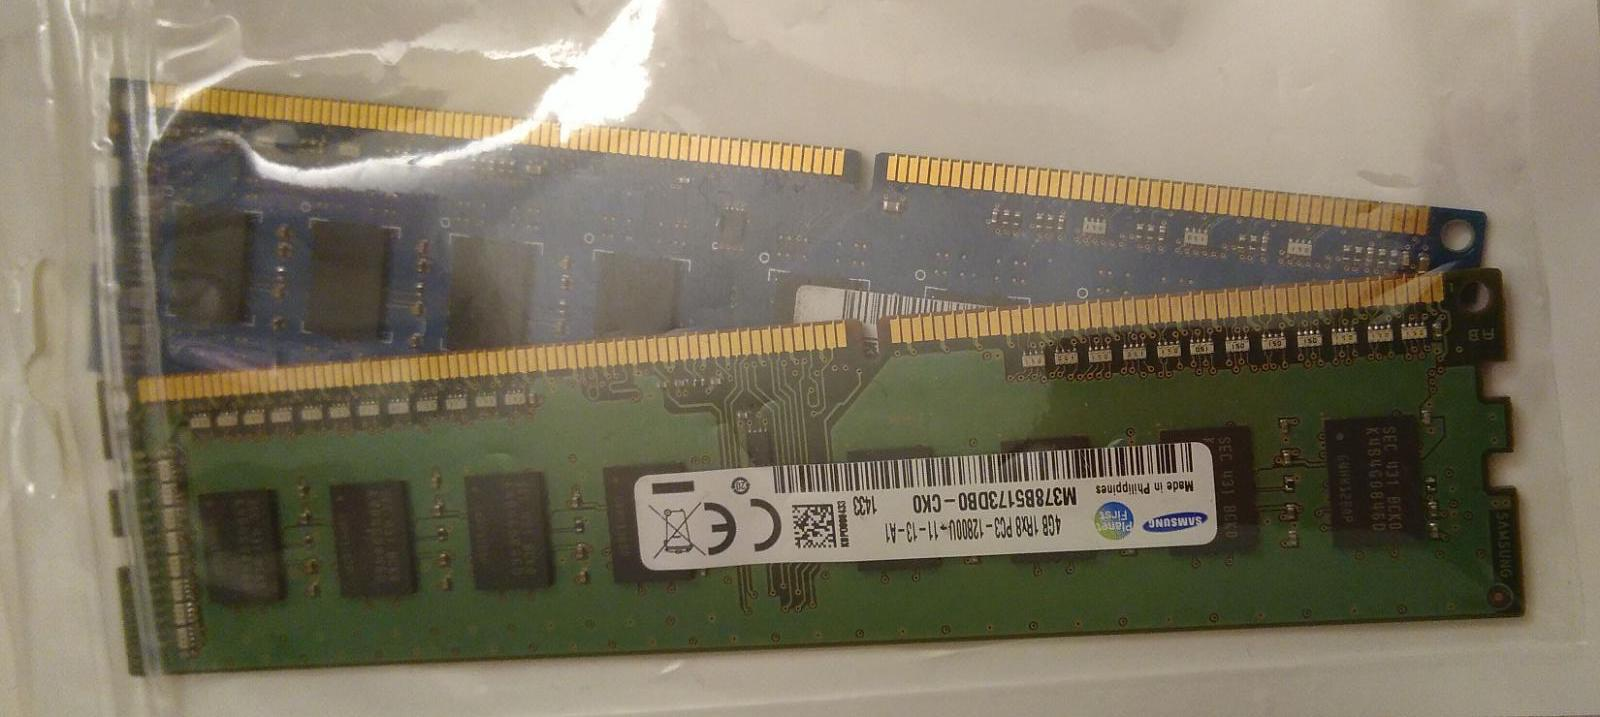
\includegraphics[width=0.8\linewidth]{RAM.jpeg}
        \caption{8Go of RAM especially bought for SPLEX Project!}
    \end{figure}
\end{frame}